% 研究過程與方法
\subsection*{一、研究架構}
本研究分為三個部分：
\begin{enumerate}
\item 建立多角度光散射量測系統與數據處理流程；
\item 量測兩種粒徑的聚苯乙烯微球懸浮液在 $\tau=0.5$ 至 $8$ 時的兩角強度比 $C$；
\item 以蒙地卡羅模擬計算相同條件下的角度分布與 $C$，並和實驗比較。
\end{enumerate}

\subsection*{二、米氏散射與異向性參數}
% 移至附錄
米氏散射描述在介質折射率為 $n$ 的空間中，波長為 $\lambda$ 的光線進入一粒徑為$d$的粒子，若符合 
\begin{equation}
    \frac{2 \pi d n}{\lambda} \approx 1
\end{equation}
則會呈現散射強度隨散射角度產生變化，符合
\begin{align}
    \mathbf{E}_s &= \sum_{n=1}^{\infty} E_n \left( i a_n \mathbf{N}^{(3)}_{e1n} - b_n \mathbf{M}^{(3)}_{o1n} \right), & \mathbf{H}_s &= \frac{k}{\omega\mu} \sum_{n=1}^{\infty} E_n \left( i b_n \mathbf{N}^{(3)}_{o1n} + a_n \mathbf{M}^{(3)}_{e1n} \right) \\
    \mathbf{E}_1 &= \sum_{n=1}^{\infty} E_n \left( c_n \mathbf{M}^{(1)}_{o1n} - i d_n \mathbf{N}^{(1)}_{e1n} \right), & \mathbf{H}_1 &= -\frac{k_1}{\omega\mu_1} \sum_{n=1}^{\infty} E_n \left( d_n \mathbf{M}^{(1)}_{e1n} + i c_n \mathbf{N}^{(1)}_{o1n} \right)
\end{align}
其中 $\mathbf{N}$、$\mathbf{N}$ 為
\begin{align}
    \mathbf{M}_{o1n} &= \cos\phi\, \pi_n z_n(\rho)\, \mathbf{e}_{\theta} - \sin\phi\, \tau_n z_n(\rho)\, \mathbf{e}_{\phi}\\
    \mathbf{M}_{e1n} &= -\sin\phi\, \pi_n z_n(\rho)\, \mathbf{e}_{\theta} - \cos\phi\, \tau_n z_n(\rho)\, \mathbf{e}_{\phi} \\
    \mathbf{N}_{e1n} &= \cos\phi\, n(n+1)\sin\theta\, \pi_n \frac{z_n(\rho)}{\rho}\, \mathbf{e}_r + \cos\phi\, \tau_n \frac{\left[\rho z_n(\rho)\right]'}{\rho}\, \mathbf{e}_{\theta} - \sin\phi\, \pi_n \frac{\left[\rho z_n(\rho)\right]'}{\rho}\, \mathbf{e}_{\phi} \\
    \mathbf{N}_{o1n} &= \sin\phi\, n(n+1)\sin\theta\, \pi_n \frac{z_n(\rho)}{\rho}\, \mathbf{e}_r + \sin\phi\, \tau_n \frac{\left[\rho z_n(\rho)\right]'}{\rho}\, \mathbf{e}_{\theta} + \cos\phi\, \pi_n \frac{\left[\rho z_n(\rho)\right]'}{\rho}\, \mathbf{e}_{\phi}
\end{align}
公式中出現的 $\pi,\ \tau,\ z$ 多項式為米氏散射中的中間公式，詳細證明請參閱\hyperlink{subsec:mie}{附錄的米氏方程導證}。
\\
本研究使用 miepython 計算兩種微球的 Mie 參數。雷射真空波長為 $\lambda=632.8\,\mathrm{nm}$，聚苯乙烯與水的折射率分別約為 $n_{\mathrm{PS}}=1.58$、$n_{\mathrm{water}}=1.332$，相對折射率為 $m=n_{\mathrm{PS}}/n_{\mathrm{water}}$。尺寸參數為 $x=2\pi r n_{\mathrm{water}}/\lambda$。計算所得尺寸參數 $x$、散射效率 $Q_{\mathrm{sca}}$ 與異向性參數 $g=\langle\cos\theta\rangle$ 如下：
\begin{center}
\begin{tabular}{cccc}
    \toprule
    粒徑 ($\mu$m) & $x$ & $Q_{\mathrm{sca}}$ & $g$ \\
    \midrule
    0.492 & 3.25 & 0.700 & 0.818 \\
    2.16 & 14.3 & 2.981 & 0.907 \\
    \bottomrule
\end{tabular}
\end{center}
$g$ 越接近 $1$，散射光越集中於前向。

\subsection*{三、穆勒矩陣與斯托克斯向量}
穆勒矩陣與斯托克向量為描述帶偏振的米氏散射方法。
斯托克向量由四項所構成，分別是總光強度$(I)$、水平與垂直線偏振差$(Q)$、正負$45$度線偏振差$(U)$、右旋與左旋圓偏振差$(V)$。
\begin{align}
    \mathbf{S} = {\left[I, Q, U, V\right]}^T
\end{align}
穆勒矩陣為瓊斯矩陣經過克羅內克積後的結果
\begin{align}
    \mathbf{M} = \mathbf{A} \left(\mathbf{J}\otimes\mathbf{J}^*\right) \mathbf{A}^{-1}
\end{align}

\subsection*{四、光學厚度}
光學厚度 $\tau$ 表示光穿過樣品時平均被散射的次數：
\[
\tau = N Q_{sca} \pi r^2 L
\]
其中 $N$ 為粒子數量濃度（個/$\mathrm{cm}^3$；表中顆/mL 數值代入前須除以 $1000$），$Q_{sca}\pi r^2$ 為一顆粒子的散射截面，
$L=1\,\mathrm{cm}$ 為比色槽光徑。$\tau\ll1$ 時大多數光子最多只被散射一次，
散射光的角度分布就是單一粒子的 Mie 相位函數；$\tau$ 增加後，光子被散
射多次，方向逐漸被打亂，角度分布也被「壓平」。光子方向被打亂所需的距離
，約為平均自由徑的 $\frac{1}{1 - g}$ 倍，稱為傳輸平均自由徑。g 越大，
需要的距離越長，因此在同一個 $\tau$ 下，大顆粒的角度分布應該被壓平得比
較慢。這就是本研究預期 $C(\tau)$ 會因粒徑而不同的物理依據。
\subsection*{五、獨立散射條件}
本研究最濃樣品的粒子平均間距約為粒徑的 $11$ 倍；粒子表面間隙與水中波長之比，對 $0.492\,\mu\mathrm{m}$ 與 $2.16\,\mu\mathrm{m}$ 微球分別約為 $10$ 與 $46$，高於相依散射開始出現的約 $0.3$ 至 $0.5$ 門檻（Baillis \& Sacadura, 2000）。樣品體積分率僅 $0.039\%$，因此將粒子視為獨立散射體；光子可以經歷多次散射，但每次散射仍以單一粒子的 Mie 理論描述。

\subsection*{六、主指標 $C$ 與角度選擇}
本研究以旋轉臂角度作為量測角度。光由比色槽壁射出時會折射，因此臂角與水中的散射角不同；蒙地卡羅模擬納入此折射，實驗與模擬皆以臂角比較。比較不同前向與後向角度組合後，依據數據穩定性、粒徑區別度、對 $\tau$ 的敏感度及與模擬的接近程度，選用
\[
C=\frac{I(30^\circ)}{I(125^\circ)}.
\]
原先使用的 $I(41.8^\circ)/I(138.2^\circ)$ 僅作為對照。

\subsection*{七、樣品配製}
\textbf{(一) 母液數量濃度}\\
兩種聚苯乙烯微球母液的質量濃度皆為 $c=25\,\mathrm{mg/mL}=0.025\,\mathrm{g/mL}$。以聚苯乙烯密度 $\rho\approx1.05\,\mathrm{g/cm^3}$，並假設微球為直徑 $d$ 的球體，母液數量濃度由
\[
N_0=\frac{c}{\rho\,(\pi d^3/6)}
\]
換算，$0.492\,\mu\mathrm{m}$ 微球約為 $3.82\times10^{11}$ 顆/mL，$2.16\,\mu\mathrm{m}$ 微球約為 $4.51\times10^9$ 顆/mL。

\medskip
\noindent\textbf{(二) 稀釋與配製}\\
每槽總體積為 $4000\,\mu\mathrm{L}$，以微量吸管取母液並加去離子水稀釋。各目標光學厚度所需的母液體積及對應數量濃度列於表中。$\tau=1$ 時，兩種微球的數量濃度分別約為 $7.5\times10^8$ 顆/mL 與 $9.2\times10^6$ 顆/mL。母液最少取用 $3.9\,\mu\mathrm{L}$；吸管最小刻度為 $0.1\,\mu\mathrm{L}$，僅刻度造成的相對誤差約為 $3\%$，實際取液誤差可能更大。另以純水配製空白樣品。

\begin{table}[H]
\centering
\caption{不同目標光學厚度的母液用量與數量濃度}
\label{tab:dilution}
\small
\renewcommand{\arraystretch}{1.2}
\begin{tabular}{c|rrrrrr}
    \toprule
    $\tau$ & 0.5 & 1 & 2 & 4 & 6 & 8 \\
    \midrule
    $0.492\,\mu\mathrm{m}$ 母液 ($\mu\mathrm{L}$) & 3.9 & 7.9 & 15.7 & 31.5 & 47.2 & 63.0 \\
    $2.16\,\mu\mathrm{m}$ 母液 ($\mu\mathrm{L}$) & 4.1 & 8.1 & 16.2 & 32.5 & 48.7 & 65.0 \\
    $0.492\,\mu\mathrm{m}$ 數量濃度 ($10^8$ 顆/mL) & 3.8 & 7.5 & 15 & 30 & 45 & 60 \\
    $2.16\,\mu\mathrm{m}$ 數量濃度 ($10^6$ 顆/mL) & 4.6 & 9.2 & 18 & 37 & 55 & 73 \\
    \bottomrule
\end{tabular}
\end{table}

\subsection*{八、實驗量測與數據處理}
\subsubsection*{(一) 量測方式}
\begin{enumerate}
    \item 架設暗室以阻隔環境光，將裝有樣品的方形比色槽放在以雙面膠標示的固定位置。
    \item 調整旋轉臂角度與高度，使直射光剛好照到感測器，並以此位置定為 $0^\circ$。比色槽面向雷射，使槽壁大致垂直於雷射光、但略向前傾，避免反射光直接返回雷射而影響輸出。
    \item 關閉雷射，量測暗室背景與暗讀值；暗室環境亮度確認低於 $0.001\,\mathrm{lux}$。
    \item 開啟雷射後，旋轉臂每次轉動 $1^\circ$ 並停留約 $2$ 秒；含馬達與程式執行時間，每格實測週期約 $2.45$ 秒。旋轉臂由 $0^\circ$ 量至 $140^\circ$ 後返回原位，為一輪；每個樣品量測兩輪，約需 $12$ 分鐘。
    \item 回到 $0^\circ$ 時比對初始讀值，以確認旋轉臂是否回到原位。依 Stokes 定律估算，$2.16\,\mu\mathrm{m}$ 微球在水中的沉降速度約 $0.5\,\mathrm{mm/h}$，一次量測期間沉降約 $0.1\,\mathrm{mm}$，可忽略。
\end{enumerate}
\begin{figure}[H]
    \centering
    % 左邊的照片（寬度設為版面的 48%）
    \begin{subfigure}[b]{0.48\textwidth}
        \centering
        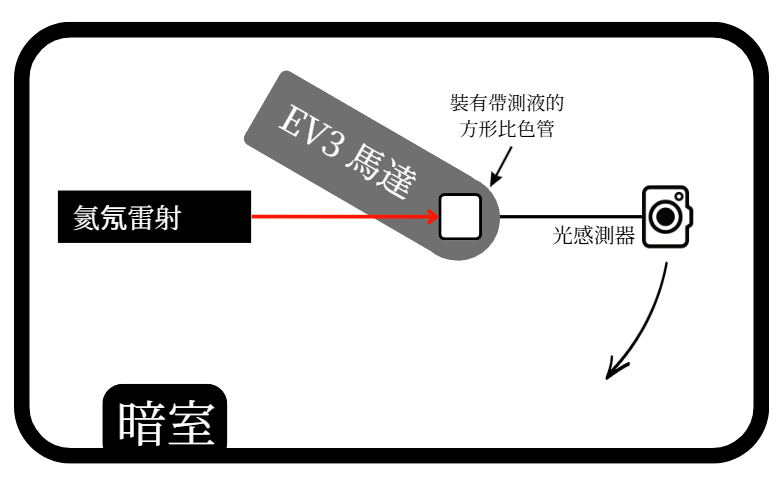
\includegraphics[width=\textwidth]{image/structure.png}
        \caption{裝置實照}\label{fig:left}
    \end{subfigure}
    \hfill 
    \begin{subfigure}[b]{0.48\textwidth}
        \centering
        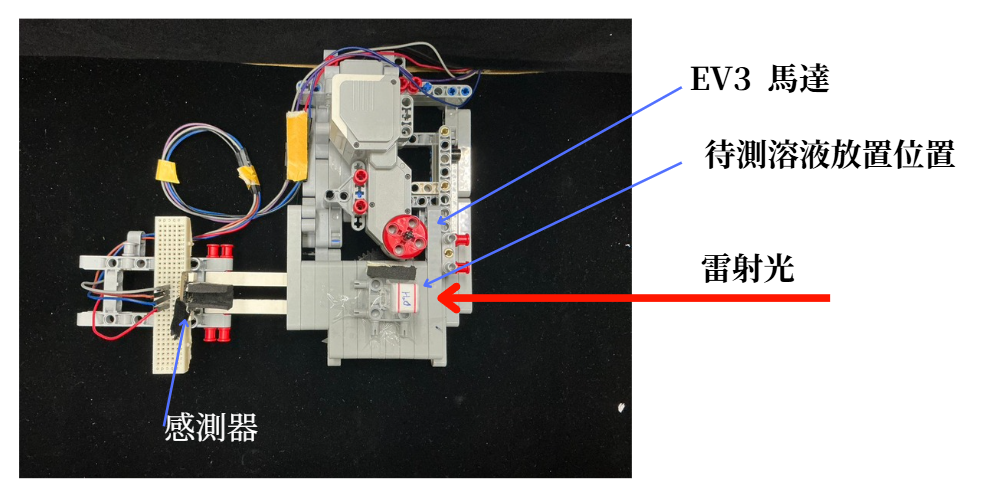
\includegraphics[width=\textwidth]{image/structure_image.png}
        \caption{裝置示意圖}\label{fig:right}
    \end{subfigure}\label{fig:both}
\end{figure}

\subsubsection*{(二) 感測器增益與空白量測}
感測器增益與積分時間由韌體依讀值切換：預設為 HIGH 增益、積分時間 $600\,\mathrm{ms}$；全光譜通道 CH0 低於 $5000$ 時，切換至 MAX 增益、$200\,\mathrm{ms}$，並維持至 CH0 超過 $50000$ 或飽和後才切回 HIGH，以減少頻繁切換。若 HIGH 飽和，則改以 MED 增益、$100\,\mathrm{ms}$ 補讀一筆，該筆不納入分析。依規格書，HIGH 與 MAX 的典型增益分別約為 LOW 的 $400$ 倍與 $9200$ 倍；同型晶片的 HIGH 增益範圍約為 $360$ 至 $440$ 倍，MAX 約為 $8500$ 至 $9900$ 倍（ams-OSRAM AG, 2023）。量測當天於不同時段各量一次純水空白，並量測雷射關閉時的暗讀值。

\subsubsection*{(三) 數據監測方式}
以 Rust 撰寫監測程式，持續讀取 Arduino 的序列埠資料並存成 CSV，以供後續處理。

\subsubsection*{(四) 數據處理}
\begin{enumerate}
    \item 僅保留完整讀值列；剔除飽和讀值、增益切換後的第一筆，以及偏離中位數超過 $4$ 倍穩健標準差的離群值。
    \item 依實測步進週期 $2.45$ 秒推算每個角度格的時間區間，只保留整段曝光都發生在旋轉臂靜止期間的讀值，每格取中位數。
    \item 由每格時間推定臂角（每格 $1^\circ$），再依當天記錄修正角度零點。
    \item 將 HIGH 讀值乘以倍率 $r$，換算為 MAX 等效讀值。依兩種設定的典型增益與積分時間估算，$r=(9200/400)\times(200/600)\approx7.7$；考量晶片個體差異，以旋轉臂靜止且同一格同時有兩種增益讀值的位置，取 MAX 與 HIGH 中位數之比實測，得到 $r=7.48$。此值落在規格範圍內；$30^\circ$ 與 $125^\circ$ 均以 MAX 量得，因此 $C$ 不受此換算影響。
    \item 扣除第二次量測的純水空白，計算淨強度
    \[
        I_{\mathrm{net}}(\theta)=I_{\mathrm{sample}}(\theta)-I_{\mathrm{blank}}(\theta).
    \]
    \item 每輪分別計算 $C=I_{\mathrm{net}}(30^\circ)/I_{\mathrm{net}}(125^\circ)$，再取兩輪平均。
    \item 不確定度取三項平方和開根號：兩輪 $C$ 差的一半、改用另一次純水空白所造成差異的一半，以及角度整體偏移 $\pm0.5^\circ$ 所造成差異的一半。
\end{enumerate}

\subsection*{九、蒙地卡羅模擬}
本研究以蒙地卡羅模擬計算理想條件下（不含雜散光與量測雜訊）的角度分布，作為實驗對照。每顆光子自比色槽入口射入，先依
\[
s=-\frac{\ln\xi}{\mu_s}
\]
前進隨機距離，其中 $\xi$ 為 $0$ 至 $1$ 之間的亂數，$\mu_s$ 為散射係數；碰到微球後，依含粒徑分布的 Mie 相位函數決定新方向，粒徑分布的變異係數分別採用 $0.492\,\mu\mathrm{m}$ 的 $2.1\%$ 與 $2.16\,\mu\mathrm{m}$ 的 $3.1\%$。光子碰到比色槽壁時，依 Fresnel 公式處理水、PMMA（折射率 $1.489$）與空氣界面的反射及透射，包含槽壁內多次反射與全反射；穿出後再依 Snell 定律折射，記錄其落入旋轉臂的 $1^\circ$ 角度格。

每個 $\tau$ 模擬 $5{,}000$ 萬顆光子；光子偏離光束平面超過 $150\,\mathrm{mm}$ 後停止追蹤。模擬假設雷射為非偏振光，旋轉臂半徑取實測值 $110\,\mathrm{mm}$，並以遮光管收光半角 $15.3^\circ$（管長 $11\,\mathrm{mm}$、開口寬 $6\,\mathrm{mm}$）限制感測器收光。每個條件使用 $6$ 組不同亂數種子，取模擬平均值，再以和實驗相同的方式計算 $C$。驗證時，移除比色槽、令 $\tau\to0$ 並只計入單次散射光子，模擬結果與 Mie 理論一致；另以獨立重寫的程式計算六個條件，結果在統計誤差內一致。